\chapter{Stability}
\label{appendix1-ade}

The non-autonomous system of coupled differential equations (\ref{eq:de-cont})--(\ref{eq:de-eul}) for density and velocity perturbations can be written as
\be 
\vec{\mathbf{x}}' = \mathbf{B}(a;\theta_j) \, \vec{\mathbf{x}}\, ,
\label{eq:appendix:B1}
\ee
where $ \vec{\mathbf{x}}^\intercal = (\delta_m,\, V_m,\, \delta_{de},\, V_{de}) $, $ \mathbf{B} $ is a $ 4\times4 $ matrix which depends on the parameters $\theta_j=\lcb H_0,\, w,\, \Omega_m,\, \Omega_x,\,  c_s,\, \aa,\, \ff,\, \gg \rcb$, on the mode $ k $ and the scale factor $ a $. In order to obtain information about the parameter space, we assess the stability of the system (\ref{eq:appendix:B1}). We compute the eigenvalues $ \lambda_k (a,\, \theta_j)$ of the matrix $\mathbf{B}(a;\theta_j)$ numerically and look at the regions in the $\theta_j-$space where all eigenvalues have negative real parts for the whole time interval we consider, that is, from matter domination to the present time. 

For the system (\ref{eq:appendix:B1}) we find one eigenvalue which does not have a region in $\theta_j-$space where $\operatorname{Re} \left( \lambda_k (a,\, \theta_j) \right) < 0$. Then, since we know that in matter dominated era and on sub-horizon scales matter perturbations grow linearly, that is, $ \delta_m \propto a$, we use the following approach to assess the stability of the system. First, we rescale the  variables $ \vec{\mathbf{x}} $ dividing them by a power $ a^m $ of the scale factor, $\vec{\mathbf{y}}=a^{-m}\vec{\mathbf{x}}$. It follows that the system  (\ref{eq:appendix:B1}) becomes   
\be
\vec{\mathbf{y}}' = \mathbf{A}(a;\theta_j) \, \vec{\mathbf{y}}\, ,
\label{eq:appendix:B2}
\ee
where $ \mathbf{A}(a;\theta_j) = \mathbf{B}(a;\theta_j) - \frac{m}{a} \mathbf{I}  $, with $ \mathbf{I} $ the identity matrix. Second, we find regions in parameter space where all the eigenvalues of the matrix $ \mathbf{A} $ have negative real parts. We study models with $ \aa=\gg=0 $ since the effective sound speed $ \ceff^2 $ is only defined in terms of $ c_s $ and $ \ff $;  moreover we check the robustness of our method with different powers $ m $. Figure \ref{fig:stability} shows regions where all eigenvalues have real part negative in the time interval relevant for both super and sub-horizon scales.  Since we use $ c_s^2=1 $ we can see clearly an upper limit on $ \ff =3/2$, which nicely agrees with $ \ceff^2>0 $.  

\begin{figure}[tb]
\centering
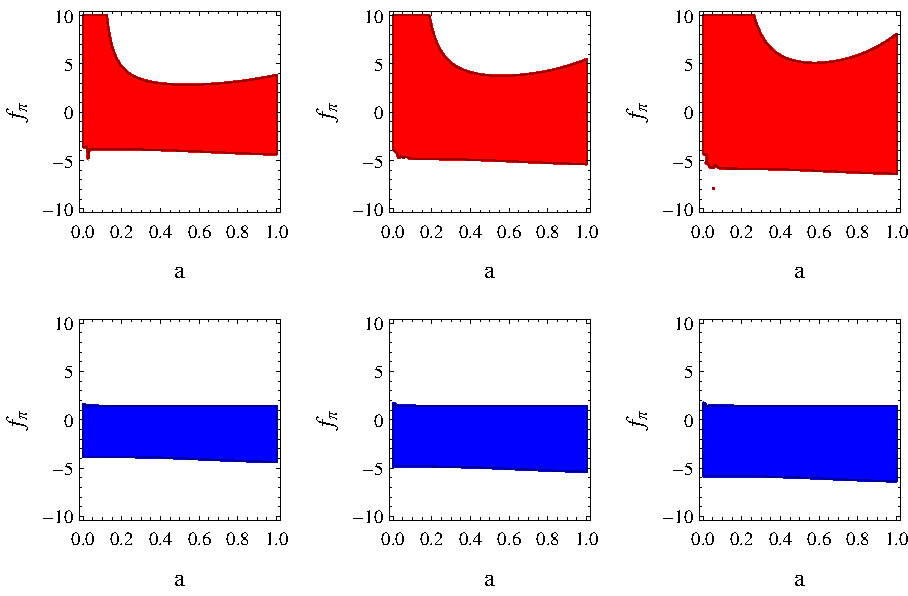
\includegraphics[width=\textwidth]{figures/chapter-ade/stability.pdf} 
\caption{The figure shows the region in the $ \ff-$space for which all the eigenvalues of the matrix $ \mathbf{A} $ in Eq. (\ref{eq:appendix:B2}) have negative real parts. The red region (upper panel) corresponds to a mode on super-horizon scales ($k=5 H_0$) in matter domination. The blue region (lower panel) shows a sub-horizon mode  ($ k=300 H_0 $). We have used $c_s^2 = 1$, $w=-1.05$, $\aa=0$ and $\gg=0$. In each column, from left to right, we rescale the variables by using powers $ m=2,\,3,\,4 $.}
\label{fig:stability}
\end{figure}

Then we study the impact of the parameter $ \gg $ on the stability of the system. For a given scale factor $ a $ we determine regions in the plane $ \ceff-\ff $ for which the system (\ref{eq:appendix:B2}) is stable for both $ \gg \mug 1 $ and $ \gg \ll 1 $. Figure \ref{fig:stability:2} shows again the stable regions for large and small scales. 

\begin{figure}[tb]
\centering 
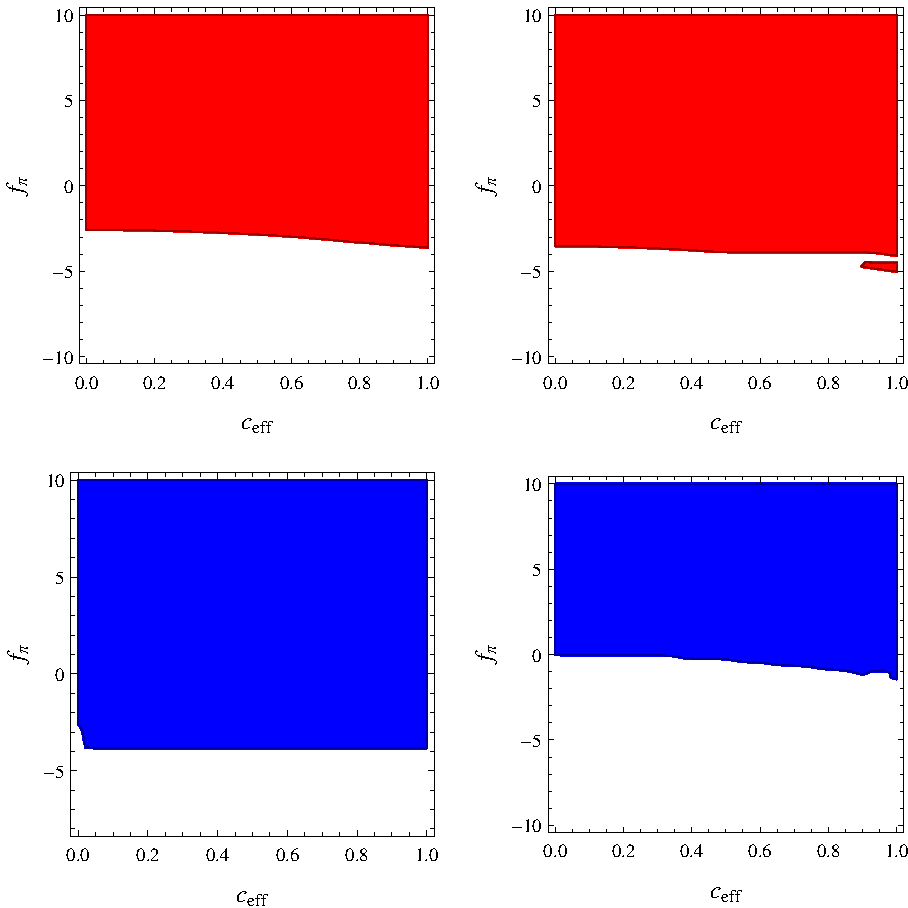
\includegraphics[width=\textwidth]{figures/chapter-ade/stability2.pdf} 
\caption{Stability regions: parameter regions where the perturbations grow more slowly than $a^2$ at $a=5\times10^{-2}$, for $w=-1.05$ and $\aa=0$. The upper row (red contours) are for $k=5 H_0$, while the lower row (blue contours) is for $k=300 H_0$. The right panels are for $ \gg = 10^{-5} $ and the left panels for $ \gg=10^5 $.}
\label{fig:stability:2}
\end{figure} 